\documentclass[11pt,a4paper]{article}

\usepackage{amsmath,amssymb}
\usepackage[margin=1in]{geometry}
\usepackage{physics}
\usepackage{braket}
\usepackage{hyperref}
\usepackage{graphicx}
\usepackage{enumitem}
\usepackage{listings}
\usepackage{xcolor}
\usepackage{tikz}
\usetikzlibrary{arrows.meta,positioning}

\lstset{
  basicstyle=\ttfamily\footnotesize,
  breaklines=true,
  language=Python,
  showstringspaces=false,
  keywordstyle=\color{blue},
  commentstyle=\color{gray},
}

\title{Pion qTMD and PDF Measurement\\Comprehensive Physics Note}
\author{Pyquda\_Measurement Collaboration}
\date{\today}

\begin{document}
\maketitle
\tableofcontents

%==========================================================================
\section{Physics Overview}
\label{sec:overview}
%==========================================================================

\subsection{Transverse Momentum Dependent Distributions}

Transverse momentum dependent (TMD) parton distribution functions and parton
distribution functions (PDFs) encode the three-dimensional momentum structure of
hadrons.  The TMD correlator for a quark in a hadron is defined on the light
cone,
\begin{equation}
  \Phi_{q}(x, \mathbf{k}_\perp; P, S)
  =
  \int \frac{d\xi^- d^2\xi_\perp}{(2\pi)^3}\,
  e^{i k\cdot\xi}\,
  \braket{P, S|\,
    \bar\psi(0)\, \mathcal{W}(0,\xi;\text{path})\, \psi(\xi)
  \,|P, S}
  \Big|_{\xi^+=0},
\end{equation}
where $\mathcal{W}(0,\xi;\text{path})$ is the staple-shaped Wilson line
connecting the quark fields, $P$ is the hadron momentum, and $S$ its spin.

On the lattice, we work at equal time and replace the light-cone separation
with a purely spatial displacement.  The quasi-TMD correlator in the
rest frame of the temporal direction is
\begin{equation}
  \tilde\Phi_{\Gamma}(b_\perp, b_z, p^z; \tau)
  =
  \braket{
    \pi(p^z)\,\big|\,
    \bar\psi(0)\,\Gamma\,
    \mathcal{W}_{\text{CG}}(0; b_\perp, b_z)\,\psi(\tau; b_\perp, b_z)
    \,\big|\,\pi(p^z)
  }.
\end{equation}
Here $\mathbf{b}_\perp = b_\perp\mathbf{e}_\perp$ is the transverse displacement
(in the $x$ or $y$ direction), $b_z\mathbf{e}_z$ is the longitudinal
displacement along the boost direction, $\tau$ is the operator insertion time,
and $\mathcal{W}_{\text{CG}}$ denotes the coordinate-gauge Wilson line (or a
true gauge-covariant staple for the operator with explicit gauge links).
$\Gamma$ is a Dirac matrix selecting the desired spin structure.

\subsection{Equal-Time Correlators on the Lattice}

On the Euclidean lattice the time coordinate is Wick-rotated: $t = i\tau$.
The equal-time operator insertion means the quark and antiquark fields in the
nonlocal bilinear are evaluated at the same time slice $\tau$ (or equivalently
the same Euclidean time $t$).  The spatial displacement $\mathbf{b}$ is
realized as a lattice shift operator acting on the quark propagator.

For the pion, which is a spin-zero meson, only specific $\Gamma$ projections
survive and the TMDs are spin-averaged.  The pion qTMD distribution probes
the transverse and longitudinal momentum correlations of the valence quark and
antiquark within the pion.

%==========================================================================
\section{Quasi-PDF and Quasi-TMD: LaMET Framework}
\label{sec:lamet}
%==========================================================================

Physical PDFs and TMDs are defined on the light cone, while lattice QCD
computes correlation functions at equal time.  Large momentum effective theory
(LaMET) \cite{Ji:2013dva,Ji:2014gla} bridges the two:  one computes a
\emph{quasi-distribution} on the lattice at finite hadron momentum $p^z$, then
matches it to the physical distribution through a factorization formula
\begin{equation}
  \tilde q(x, b_\perp, p^z; \mu)
  =
  \int \frac{dy}{|y|}\,
  C\!\left(\frac{x}{y}, \frac{\mu}{p^z}\right)\,
  q(y, \mu)
  + \mathcal{O}\!\left(\frac{\Lambda_{\rm QCD}^2}{(p^z)^2},
                         \frac{\Lambda_{\rm QCD}^2}{b_\perp^2}\right).
\end{equation}
The pion boost momentum $\mathbf{p}_f = (0,0,p^z)$ is a crucial parameter.
Three regimes must be controlled:
\begin{enumerate}[label=(\roman*)]
  \item The boost momentum must be large enough that power corrections
        $\Lambda_{\rm QCD}^2/(p^z)^2$ are under control.
  \item The spatial displacement $b_z$ must be small compared to the
        correlation length of the gauge links (to avoid large noise from
        Wilson line self-energy).
  \item The transverse displacement $b_\perp$ must be large enough to resolve
        non-perturbative transverse structure but small enough to avoid
        discretization effects.
\end{enumerate}

In this workflow, the quasi-TMD is computed directly from the lattice
three-point function with a nonlocal displacement operator inserted between the
source and the fixed sink.  The equal-time correlator is
\begin{equation}
  \tilde C_3^{\Gamma}(q, b_\perp, b_z; \tau; p_f, t_{\rm sep})
  =
  \sum_{\mathbf{x}}\sum_{\mathbf{y}}
  e^{-i\mathbf{q}\cdot(\mathbf{x}-\mathbf{x}_0)}\,
  e^{-i\mathbf{p}_f\cdot(\mathbf{y}-\mathbf{x}_0)}\,
  \Braket{
    \pi(\mathbf{y}, t_{\rm sep})\;
    \big|\;
    \bar\psi(\mathbf{x},\tau)\,\Gamma\,
    \mathcal{O}_{b_\perp,b_z}\,\psi(\mathbf{x},\tau)
    \big|\;
    \pi(\mathbf{x}_0, 0)
  }.
\end{equation}

The momentum $\mathbf{p}_f$ is the fixed sink momentum that determines the pion
boost; $\mathbf{q}$ is the Fourier momentum at the operator insertion; and the
initial pion momentum $\mathbf{p}_i$ is related by momentum conservation at the
insertion: $\mathbf{p}_f = \mathbf{p}_i + \mathbf{q}$ when the operator carries
zero momentum (purely spatial displacement).  In practice $p_f$ is set to the
desired boost and $q$ scans all momentum modes of the lattice for the
non-forward matrix element.

%==========================================================================
\section{Two-Point Function}
\label{sec:twopt}
%==========================================================================

\subsection{Physical Definition}

The connected pion two-point function for source gamma $\Gamma_{\rm src}$ and
sink gamma $\Gamma_{\rm sink}$ is
\begin{equation}
  C_2^{\Gamma_{\rm sink}}(p, t)
  =
  \sum_{\mathbf{x}}
  e^{-i\mathbf{p}\cdot(\mathbf{x}-\mathbf{x}_0)}\,
  \Tr_{\rm spin, color}\!\Big[
    S_{\rm anti}(\mathbf{x},t; \mathbf{x}_0,0)\,
    \Gamma_{\rm sink}\,
    S_q(\mathbf{x},t; \mathbf{x}_0,0)\,
    \Gamma_{\rm src}
  \Big],
  \label{eq:c2}
\end{equation}
where $S_q(x,y)$ is the quark propagator from source $y$ to sink $x$, and
$S_{\rm anti}$ is the antiquark line constructed via $\gamma_5$-hermiticity:
\begin{equation}
  S_{\rm anti}(x,y) = \gamma_5\, S_q(x,y)^\dagger\, \gamma_5.
\end{equation}

\subsection{Source Gamma Convention}

The default source gamma is the explicit canonical label \texttt{5}, which
sets $\Gamma_{\rm src}=\gamma_5$ for all sink channels and corresponds to
the standard pseudoscalar pion interpolator
$\bar\psi \gamma_5 \psi$.  The shared source-Gamma utility supports:
\begin{itemize}[nosep]
  \item Any of the 16 canonical Gamma labels: the selected source matrix is
        fixed while all 16 sink channels are scanned.
  \item \texttt{dagger\_of\_sink}: $\Gamma_{\rm src}
        = \gamma_5 \Gamma_{\rm sink}^\dagger \gamma_5$.
\end{itemize}
The former aliases \texttt{fixed\_g5} and \texttt{same\_as\_sink} are not
accepted.  Explicit \texttt{5} replaces \texttt{fixed\_g5} without changing
the numerical contraction.  The relational \texttt{dagger\_of\_sink} mode
is used by qDA local C2; it produces 16 paired source/sink channels rather than
a fixed-source sink scan.
For an explicit pseudoscalar source, output provenance uses
\texttt{source\_gamma\_mode=fixed},
\texttt{source\_gamma\_label=5}, and the filename channel tag
\texttt{.src5}.

All 16 sink gamma matrices are scanned and stored, ordered as
\begin{equation}
  \label{eq:gamma_order}
  \gamma_5,\;
  \gamma_T,\;
  \gamma_T\gamma_5,\;
  \gamma_X,\;
  \gamma_X\gamma_5,\;
  \gamma_Y,\;
  \gamma_Y\gamma_5,\;
  \gamma_Z,\;
  \gamma_Z\gamma_5,\;
  I,\;
  \Sigma_{XT},\;
  \Sigma_{XY},\;
  \Sigma_{XZ},\;
  \Sigma_{YT},\;
  \Sigma_{YZ},\;
  \Sigma_{ZT},
\end{equation}
corresponding to PyQUDA gamma indices
$[15, 8, 7, 1, 14, 2, 13, 4, 11, 0, 9, 3, 5, 10, 6, 12]$.

\subsection{Einsum Contraction Pattern}

The array layout of a PyQUDA propagator is
\begin{equation}
  \texttt{prop.data}[w,\, t,\, z,\, y,\, x_{\rm cb},\,
                      \text{spin}_{\rm sink},\,
                      \text{spin}_{\rm src},\,
                      \text{color}_{\rm sink},\,
                      \text{color}_{\rm src}],
\end{equation}
where $w$ is the even-odd parity index (checkerboard), $t,z,y,x_{\rm cb}$
are space-time coordinates, and the remaining four indices carry spin and color.

The antiquark line is constructed as (\verb|_meson_backward_line|):
\begin{equation}
  \texttt{bw\_prop}[w,t,z,y,x_{\rm cb},j,i,b,a]
  =
  (\gamma_5)_{k i}\,
  \texttt{prop.data}[w,t,z,y,x_{\rm cb},l,a,b]^*
  (\gamma_5)_{l j}.
\end{equation}

The contraction proceeds in two einsum steps:
\begin{enumerate}[nosep]
  \item Attach sink gamma to backward line:
  \begin{equation}
    \texttt{bw\_prop}_{\Gamma}[g,w,t,z,y,x_{\rm cb},j,m,c,f]
    =
    \texttt{bw\_prop}[w,t,z,y,x_{\rm cb},j,i,c,f]\,
    (\Gamma_g)_{i m}.
  \end{equation}
  \item Full contraction with source gamma and color/spin trace:
  \begin{align}
    \texttt{corr\_local}[g,w,t,z,y,x_{\rm cb}]
    &=
    \texttt{bw\_prop}_{\Gamma}[g,w,t,z,y,x_{\rm cb},j,i,a,b]\;
    \texttt{prop\_f.data}[w,t,z,y,x_{\rm cb},l,b,a]\;
    (\Gamma_{\rm src})_{l j}.
  \end{align}
\end{enumerate}

The momentum phase is applied via a Fourier-phase tensor
$\texttt{phases}[q, w, t, z, y, x_{\rm cb}]$ generated by
\verb|MomentumPhase.getPhases| with momentum arguments $p_{\rm xyz}$ and source
position $x_0$.  The phase convention in the code uses $e^{-i\mathbf{p}\cdot
(\mathbf{x}-\mathbf{x}_0)}$: for the two-point function, negated three-momenta
$[-p_x, -p_y, -p_z]$ are passed to the phase generator, so that
\begin{equation}
  \texttt{phases}[q,w,t,z,y,x_{\rm cb}]
  \;\widehat{=}\;
  e^{-i\mathbf{p}_q\cdot(\mathbf{x}-\mathbf{x}_0)}.
\end{equation}
The final momentum-projected correlator is
\begin{equation}
  \texttt{corr}[g,q,t]
  =
  \sum_{w,z,y,x_{\rm cb}}
  \texttt{phases}[q,w,t,z,y,x_{\rm cb}]\;
  \texttt{corr\_local}[g,w,t,z,y,x_{\rm cb}].
\end{equation}

\subsection{Boosted Smearing}

Two source-smeared, point-sink propagators are defined by
\begin{equation}
 Q_{+}^{SP}=D^{-1}\mathcal S_{+}\delta_{x_0},\qquad
 Q_{-}^{SP}=D^{-1}\mathcal S_{-}\delta_{x_0}.
 \label{eq:qtmd_source_lines}
\end{equation}
The positive line is the spectator and the negative line is the active
operator line.  Equal boosts require one inversion and a copy; unequal boosts
require two independent inversions.  For the two-point function they are
boosted-smeared at the sink using their corresponding endpoint kernels:
\begin{align}
  Q_+^{SS} &\leftarrow \text{boosted\_smearing}(Q_+^{SP},
                      w, \texttt{pos\_boost}), \\
  Q_-^{SS} &\leftarrow \text{boosted\_smearing}(Q_-^{SP},
                      w, \texttt{neg\_boost}).
\end{align}
The implementation in \verb|boosted_smearing_pyquda.py| uses a spatial
FFT convolution with the real-space kernel
\begin{equation}
  K_{\mathbf{k}}(\mathbf{r})
  =
  \exp\!\left(-\frac{r_x^2+r_y^2+r_z^2}{2w^2}\right)
  \exp\!\left[
    2\pi i
    \left(
      \frac{k_x r_x}{L_x}
      + \frac{k_y r_y}{L_y}
      + \frac{k_z r_z}{L_z}
    \right)
  \right].
  \label{eq:qtmd_smear_kernel}
\end{equation}
Here \(\mathbf{k}=(k_x,k_y,k_z)\) is the integer vector supplied by
\texttt{pos\_boost} or \texttt{neg\_boost}, while \(\mathbf{r}\) is the centered
periodic global coordinate on the current MPI rank.  For each spin-color column
of a fermion or propagator the smeared field is
\begin{equation}
  \psi^{\,{\rm smear}}_{\mathbf{k}}(\mathbf{x},t)
  =
  \mathcal{F}^{-1}_{3d}
  \left[
    \mathcal{F}_{3d}[\psi](\mathbf{p},t)\,
    \mathcal{F}_{3d}[K_{\mathbf{k}}](\mathbf{p})
  \right](\mathbf{x},t).
  \label{eq:qtmd_fft_smear}
\end{equation}
The FFT is three-dimensional and spatial only; the same kernel is applied on
each Euclidean time slice.  The current implementation assumes identity gauge
for this smearing step, i.e. no explicit gauge rotation is applied before or
after the FFT.

%==========================================================================
\section{Three-Point qTMD Function (Pre-Sequential-Trick)}
\label{sec:threept}
%==========================================================================

\subsection{Physical Correlator}

The connected pion qTMD three-point function, before applying the sequential
source trick, reads
\begin{equation}
  \boxed{
  \begin{aligned}
    C_3^{\Gamma}(q, b_\perp, b_z; \tau; p_f, t_{\rm sep})
    &=
    \sum_{\mathbf{x}}\sum_{\mathbf{y}}
    e^{-i\mathbf{q}\cdot(\mathbf{x}-\mathbf{x}_0)}\,
    e^{-i\mathbf{p}_f\cdot(\mathbf{y}-\mathbf{x}_0)} \\
    &\qquad\times
    \Tr_{\rm spin, color}\Big[
      S_{\rm anti}(\mathbf{y},t_{\rm sep}; \mathbf{x}_0,0)\,
      \Gamma_{\rm sink}\,
      S_q(\mathbf{y},t_{\rm sep}; \mathbf{x},\tau)\,
      \Gamma_{\rm ins}\,
      \mathcal{O}_{b_\perp,b_z}\,
      S_q(\mathbf{x},\tau; \mathbf{x}_0,0)\,
      \Gamma_{\rm src}
    \Big].
  \end{aligned}}
  \label{eq:c3_full}
\end{equation}
Here $\mathcal{O}_{b_\perp,b_z}$ is the nonlocal displacement operator acting on
the forward quark line.  Unlike the pion electromagnetic form factor (EMFF),
where the insertion is a local current at a single space-time point, the qTMD
insertion is nonlocal in space: the quark field at $(\tau,\mathbf{x})$ is
shifted by $(b_\perp\mathbf{e}_\perp + b_z\mathbf{e}_z)$.  This is the defining
difference from the EMFF three-point function.

The momenta satisfy $\mathbf{p}_i$ (initial), $\mathbf{p}_f$ (final sink), and
$\mathbf{q}$ (insertion) with $\mathbf{q} = \mathbf{p}_f - \mathbf{p}_i$ in the
forward matrix element.

\subsection{Why the Sequential Trick is Needed}

Computing Eq.~\eqref{eq:c3_full} directly would require a separate propagator
inversion for every $(\mathbf{q}, b_\perp, b_z, \tau)$ combination, which is
prohibitively expensive.  The fixed-sink sequential source method absorbs the
entire sink sum (over $\mathbf{y}$) into a single propagator inversion, after
which the insertion-side contraction becomes a simple two-point-like
correlation.

%==========================================================================
\section{Sequential Source}
\label{sec:sequential}
%==========================================================================

\subsection{Meson Sequential Source Construction}

The meson fixed-sink sequential source is built in
\verb|create_meson_bw_seq_pyquda|.  Given the sink-smeared propagator
$Q_+^{SS}$ (the positive-boost spectator, already positive-boost smeared at
the sink), the source
position $x_0$, the sink momentum $p_f$, the sink-source separation $t_{\rm
sep}$, and the sink Dirac matrix $\Gamma_{\rm sink}$, the right-hand side is
placed on the sink time slice $t_{\rm sink} = t_0 + t_{\rm sep}$:
\begin{align}
  \eta_{\rm seq}(\mathbf{y}; p_f, t_{\rm sep})
  &=
  \delta_{t_y,\, t_{\rm sink}}\;
  \Phi_{p_f}(\mathbf{y} - \mathbf{x}_0)\;
  \Gamma_{\rm seq}\,
  S_q(\mathbf{y},t_{\rm sink}; \mathbf{x}_0,0),
  \label{eq:eta_seq}
  \\
  \Gamma_{\rm seq}
  &=
  \gamma_5\, \Gamma_{\rm sink}^\dagger\, \gamma_5.
  \label{eq:gamma_seq}
\end{align}

The phase function $\Phi_{p_f}(\mathbf{r}) = e^{-i\mathbf{p}_f \cdot
\mathbf{r}}$ is generated by \texttt{MomentumPhase.getPhases} with the same
sign convention as the two-point function.  The time slice restriction is
enforced by \verb|pyquda_utils.source.sequential12|, which masks all time
slices except $t_{\rm sink}$.

For the smeared-smeared three-point function, the source above is smeared once
more before the sequential inversion:
\begin{equation}
  \eta_{\rm seq}^{SS}
  =
  \mathcal{S}_{w,\mathbf{k}_{\rm neg}}
  \left[
    \delta_{t_y,\, t_{\rm sink}}\;
    \Phi_{p_f}(\mathbf{y}-\mathbf{x}_0)\;
    \Gamma_{\rm seq}\,
    Q_+^{SS}(\mathbf{y},t_{\rm sink};\mathbf{x}_0,0)
  \right].
  \label{eq:qtmd_eta_seq_smear}
\end{equation}
The input line $Q_+^{SS}$ carries the positive spectator endpoint smearing.
The outer $\mathcal{S}_{w,\mathbf{k}_{\rm neg}}$ supplies the negative active
endpoint smearing absorbed into the sequential propagator.  At the operator
insertion the bilocal displacement or Wilson transporter acts on
$Q_-^{SP}$; the insertion itself is not Gaussian smeared.  This is the same
line convention used by connected pion EMT.

Only the positive-spectator/negative-active orientation is produced.  The
opposite orientation requires exchanging the two complete lines, including
both source inversions and both endpoint smearings.  Swapping only one boost
does not define that second contribution.

The sequential propagator solves
\begin{equation}
  D\; S_{\rm seq}(x; x_0) = \eta_{\rm seq}(x),
\end{equation}
where $D$ is the Wilson-clover Dirac operator.  After inversion,
$\gamma_5$-hermiticity yields the backward sequential line used in contraction:
\begin{equation}
  S_{\rm seq}^{\rm anti}(x,x_0; p_f, t_{\rm sep})
  =
  \gamma_5\,
  S_{\rm seq}(x,x_0)^\dagger\,
  \gamma_5.
  \label{eq:seq_anti}
\end{equation}

\subsection{Sink-Summed Three-Point Contraction}

With the sequential propagator, the sink sum is absorbed and the three-point
function reduces to a two-point-like form:
\begin{equation}
  \boxed{
  \begin{aligned}
    C_3^{\Gamma}(q, b_\perp, b_z; \tau; p_f, t_{\rm sep})
    &=
    \sum_{\mathbf{x}}
    e^{-i\mathbf{q}\cdot(\mathbf{x}-\mathbf{x}_0)}
    \,
    \Tr_{\rm spin, color}\Big[
      S_{\rm seq}^{\rm anti}(\mathbf{x},\tau; \mathbf{x}_0,0)
      \;
      \Gamma_{\rm ins}
      \;
      \mathcal{O}_{b_\perp,b_z}\,
      S_q(\mathbf{x},\tau; \mathbf{x}_0,0)
      \;
      \Gamma_{\rm src}
    \Big].
  \end{aligned}}
  \label{eq:c3_seq}
\end{equation}

The insertion gamma $\Gamma_{\rm ins}$ scans all 16 Dirac structures (the same
set as in Sec.~\ref{sec:twopt}), while $\Gamma_{\rm src}$ is the explicit
canonical label \texttt{5} by default and $\Gamma_{\rm sink}$ is set by the application (e.g.,
$\gamma_5$ for the pseudoscalar pion).

The shared \verb|contract_pion_gamma_scan_from_backward_line| kernel mirrors the
two-point function:
\begin{align}
  \texttt{sink\_inserted}[g,w,t,z,y,x_{\rm cb},j,m,c,f]
  &=
  S_{\rm seq}^{\rm anti}[w,t,z,y,x_{\rm cb},j,i,c,f]\;
  (\Gamma_g)_{i m},
  \\
  \texttt{corr\_local}[g,w,t,z,y,x_{\rm cb}]
  &=
  \texttt{sink\_inserted}[g,w,t,z,y,x_{\rm cb},j,i,a,b]\;
  (\text{shifted\_prop})[w,t,z,y,x_{\rm cb},l,b,a]\;
  (\Gamma_{\rm src})_{l j}.
\end{align}
Here $\texttt{shifted\_prop}$ is the negative active propagator $Q_-^{SP}$
with the nonlocal displacement operator already applied (see
Sec.~\ref{sec:cg_tmd_op}).

%==========================================================================
\section{CG qTMD Operator}
\label{sec:cg_tmd_op}
%==========================================================================

\subsection{Coordinate-Gauge Displacement}

For the CG (coordinate-gauge) qTMD path, the nonlocal operator is approximated
by a simple lattice shift, with \emph{no explicit gauge link} inserted:
\begin{equation}
  \mathcal{O}_{b_\perp,b_z}\, S_q(x, x_0)
  \;=\;
  S_q\bigl(x + b_\perp \mathbf{e}_\perp + b_z \mathbf{e}_z,\; x_0\bigr).
  \label{eq:cg_shift}
\end{equation}

This corresponds to working in a gauge where the spatial links are (at least
approximately) set to unity, so the Wilson line is trivial.  The physical
interpretation is that the gauge has been fixed to a smooth gauge (e.g.,
Coulomb or Landau gauge) before the correlation function is computed.

\subsection{Transverse Direction Scan}

The transverse displacement direction $\mathbf{e}_\perp$ is scanned over the
two transverse lattice axes:
\begin{itemize}[nosep]
  \item Direction $0$: $\mathbf{e}_\perp = \mathbf{e}_x$ (stored as
        \texttt{b\_X} in HDF5).
  \item Direction $1$: $\mathbf{e}_\perp = \mathbf{e}_y$ (stored as
        \texttt{b\_Y} in HDF5).
\end{itemize}
The code contracts both directions separately with independent propagator copies
so that successive shifts remain small and error accumulation is minimized.

\subsection{Wilson Line Index Convention}

Each displacement is labeled by a four-component Wilson line index:
\begin{equation}
  \texttt{W\_index} = [b_T,\; b_z,\; \eta,\; \text{direction}],
\end{equation}
where:
\begin{itemize}[nosep]
  \item $b_T$: transverse displacement in lattice units ($0$ to
        \texttt{b\_T}).
  \item $b_z$: longitudinal displacement in lattice units (positive and
        negative, up to $\pm\texttt{b\_z}$).
  \item $\eta$: staple length parameter (set to 0 for straight-line paths in
        current implementation).
  \item $\text{direction}$: $0$ for $\mathbf{e}_x$, $1$ for
        $\mathbf{e}_y$.
\end{itemize}

The shared incremental shift operation
\verb|qtmd_operator_utils.shift_qtmd_cg| computes
\begin{equation}
  \Delta b_T = \text{round}(b_T^{\rm current} - b_T^{\rm previous}),\qquad
  \Delta b_z = \text{round}(b_z^{\rm current} - b_z^{\rm previous}),
\end{equation}
and applies $\texttt{prop\_f.shift}(\Delta b_T,
\text{direction}).\texttt{shift}(\Delta b_z, 2)$, where direction 2 is the
$z$-axis.  The $\text{round}$ function handles cases where $b_T$ or $b_z$ could
be non-integer (though in current use they are integers).

%==========================================================================
\section{PDF Operators (bT = 0)}
\label{sec:pdf}
%==========================================================================

The PDF path is the straight-$z$ special case with $b_\perp = 0$:
\begin{equation}
  \mathbf{b} = b_z\,\mathbf{e}_z.
\end{equation}

Two variants are supported, selected by the boolean parameter
\texttt{gauge\_invariant}:

\subsection{CG PDF (Coordinate Gauge)}

The CG PDF operator is identical in spirit to the CG qTMD operator
(Sec.~\ref{sec:cg_tmd_op}) but restricted to the $z$ direction:
\begin{equation}
  \mathcal{O}^{\rm CG}_{b_z}\, S_q(x,x_0)
  \;=\;
  S_q(x + b_z\mathbf{e}_z,\; x_0).
\end{equation}
No gauge links are included.  This is implemented by the same
\verb|shift_qtmd_cg| function, which applies a lattice shift in the $z$
direction (direction index 2).

\subsection{GI PDF (Gauge Invariant)}

The GI PDF operator inserts explicit gauge-covariant shifts that build up the
Wilson line incrementally.  For a unit step in the $+z$ direction:
\begin{equation}
  \psi'(x) = U_z(x)\,\psi(x + \hat{z}),
\end{equation}
and for a unit step in the $-z$ direction:
\begin{equation}
  \psi'(x) = U_{-z}(x)\,\psi(x - \hat{z})
           = U_z^\dagger(x - \hat{z})\,\psi(x - \hat{z}).
\end{equation}

The implementation in \verb|shift_propagator_pdf_gi| applies the
gauge-covariant derivative
\texttt{gauge.pure\_gauge.covDev(fermion, dir)} spin-color by spin-color:
\begin{itemize}[nosep]
  \item \texttt{covDev(fermion, 2)}: covariant shift in $+z$ ($\Delta b_z =
        +1$).
  \item \texttt{covDev(fermion, 6)}: covariant shift in $-z$ ($\Delta b_z =
        -1$).
\end{itemize}
The PyQUDA direction convention is: $0,1,2,3$ for $+x,+y,+z,+t$ and
$4,5,6,7$ for $-x,-y,-z,-t$.

An important implementation detail is that only nearest-neighbor ($\Delta b_z =
\pm 1$) incremental changes are supported.  If the ordered Wilson line list
contains a jump larger than one lattice unit, the code raises a
\texttt{ValueError} rather than silently producing an incorrect path.  This
constraint is satisfied by construction of the Wilson line index list (see
Sec.~\ref{sec:wilson_lists}).

At zero separation the local limit is common to the qTMD, CG-PDF, GI-PDF, and
EMFF contractions:
\begin{equation}
  b_T = b_z = \eta = 0,\qquad \mathbf{q}=0
  \quad\Longrightarrow\quad
  C_3^{\rm qTMD,CG}
  =
  C_3^{\rm PDF,CG}
  =
  C_3^{\rm PDF,GI}
  =
  C_3^{\rm EMFF}
  \quad\text{for the same local current } \Gamma .
  \label{eq:qtmd_local_limit}
\end{equation}
This is a useful diagnostic of the phase, gamma, and sequential-source
conventions.  In the S8T32 smoke test the \(\Gamma=\gamma_4\) local-current
datasets agree with the pion EMFF output at machine precision.

%==========================================================================
\section{Wilson Line Index Lists}
\label{sec:wilson_lists}
%==========================================================================

\subsection{TMD Wilson Line Indices}

The shared function \verb|create_cg_qtmd_wilsonline_index_lists| returns two
lists:
\texttt{index\_list\_trans0} (transverse direction 0, i.e., $x$) and
\texttt{index\_list\_trans1} (transverse direction 1, i.e., $y$).

For a given maximum displacement $(b_T^{\rm max}, b_z^{\rm max})$, the index
pairs are enumerated as:
\begin{verbatim}
for bz in 0 .. b_z:
    for bT in 0 .. b_T:
        add [bT, bz, 0, 0]   and   [bT, bz, 0, 1]
        if bz != 0:
            add [bT, -bz, 0, 0]   and   [bT, -bz, 0, 1]
\end{verbatim}
This generates all $(b_T, b_z)$ pairs in the first quadrant and
mirror-$z$ half of the $(b_T, b_z)$ plane.  Both positive and negative $b_z$
are included to capture the full Fourier range for the $z$-direction momentum
projection.

\subsection{Reordering for Minimal Adjacent Differences}

After enumeration, an internal helper in
\verb|qtmd_operator_utils.py| reorders each list to minimize the maximum
absolute difference in $(b_T, b_z)$ between adjacent indices.  The algorithm:
\begin{enumerate}[nosep]
  \item Sort by $(b_T, b_z)$ lexicographically.
  \item Walk through the sorted list; if the jump from index $i$ to $i+1$
        exceeds one lattice unit in either coordinate, search ahead for a
        closer candidate and swap it into position $i+1$.
\end{enumerate}
This greedy reordering reduces the cumulative lattice displacement traversed
during incremental propagator shifts, which minimizes numerical noise
accumulation and improves code efficiency since smaller shifts are cheaper in
the PyQUDA propagator implementation.

\subsection{PDF Wilson Line Indices}

The shared function \verb|create_pdf_wilsonline_index_list| returns a single
list (because $b_T = 0$ always):
\begin{verbatim}
for bz in 0 .. b_z:
    add [0, bz, 0, 0]
for bz in 0 .. b_z:    # skip bz=0 (already added above)
    if bz != 0:
        add [0, -bz, 0, 0]
\end{verbatim}
The list starts at $b_z=0$ (the unshifted propagator) and incrementally walks
out to $\pm b_z^{\rm max}$ in unit steps.  Since $b_T$ is identically zero and
the $b_z$ changes are by construction $\pm 1$ or $0$ (resetting to $b_z=0$
between the positive and negative branches), no reordering is needed.

For the GI PDF path, the reset to $b_z=0$ between branches is essential: it
restarts the propagator from the original (unshifted) copy and builds the
negative-$b_z$ branch from scratch, avoiding cumulative gauge-link noise from
traversing the entire length $+b_z^{\rm max}$ to $-b_z^{\rm max}$.

%==========================================================================
\section{Code Implementation Details}
\label{sec:code}
%==========================================================================

The core implementation resides in
\verb|pyquda_measurement_utils/pion_qTMD_vibe_develop.py|, in the class
\verb|pion_TMD|.  Below we document each major method.

\subsection{\texttt{\_\_init\_\_(parameters)}}

Constructs the lightweight contraction object from a parameter dictionary
with keys:
\begin{itemize}[nosep]
  \item \texttt{p\_2pt}: momentum list for the two-point function.
  \item \texttt{width}: Gaussian smearing width.
  \item \texttt{pos\_boost}, \texttt{neg\_boost}: boosted smearing momentum
        boosts for quark and antiquark lines.
\end{itemize}
The application layer owns $\eta$, $b_z$, $b_T$, insertion momenta,
$t_{\rm sep}$, and output scheduling.  It constructs the Wilson-index lists
with the neutral \verb|qtmd_operator_utils| functions and passes them to the
contraction object.

\subsection{\texttt{contract\_2pt\_pion}}

\begin{lstlisting}
def contract_2pt_pion(self, latt_info, spectator_prop, active_prop, phases, tag,
                       src_gamma="5"):
\end{lstlisting}

Workflow:
\begin{enumerate}[nosep]
  \item Sink-smear \texttt{spectator\_prop} with \texttt{pos\_boost} and
        \texttt{active\_prop} with \texttt{neg\_boost}.
  \item Call the shared pion C2 kernel, which constructs the
        $\gamma_5$-hermitian backward line, scans the 16 sink Gamma channels
        one at a time, Fourier-projects, and gathers across MPI ranks.
  \item Save to HDF5 via \texttt{save\_proton\_c2pt\_hdf5}.
\end{enumerate}

The output shape is \texttt{[gamma, momentum, time]}.

\subsection{\texttt{contract\_qTMD\_CG}}

\begin{lstlisting}
def contract_qTMD_CG(self, latt_info, active_prop, seq_bw_prop, phases,
                      W_index_list_dir0, W_index_list_dir1,
                      src_gamma="5"):
\end{lstlisting}

Workflow:
\begin{enumerate}[nosep]
  \item Prepare gamma stacks ($\Gamma_g$ and $\Gamma_{\rm src}$) and phases.
  \item Construct sequential backward line
        $\texttt{seq\_bw\_line} = \gamma_5\,
        \texttt{seq\_bw\_prop}^\dagger \gamma_5$.
  \item For direction 0 ($x$): iterate over \texttt{W\_index\_list\_dir0},
        incrementally shifting the negative active propagator using
        \verb|shift_qtmd_cg| and contracting at each step via
        the shared Gamma-scan kernel.
  \item Reset and repeat for direction 1 ($y$) with
        \texttt{W\_index\_list\_dir1}.
  \item Stack all results into a numpy array.
\end{enumerate}

Each Wilson index produces an output of shape \texttt{[gamma, momentum, time]};
stacking across all $N_W$ Wilson indices yields shape \texttt{[N\_W, gamma,
momentum, time]}.

The per-shift kernel deliberately does not construct a
\texttt{[16,propagator]} object.  It retains only one propagator-sized
Gamma-inserted line at a time and accumulates the small
\texttt{[gamma,momentum,time]} result.

\subsection{\texttt{contract\_PDF}}

\begin{lstlisting}
def contract_PDF(self, latt_info, gauge, active_prop, seq_bw_prop, phases,
                  W_index_list, src_gamma="5",
                  gauge_invariant=True):
\end{lstlisting}

Same structure as \verb|contract_qTMD_CG| but:
\begin{itemize}[nosep]
  \item Uses a single \texttt{W\_index\_list} (no transverse direction
        separation).
  \item Resets the negative active propagator to the original copy whenever $b_z$
        returns to $0$ (handling the split between positive and negative
        branches).
  \item Calls \verb|shift_propagator_pdf_gi| when
        \texttt{gauge\_invariant=True} or \verb|shift_qtmd_cg| when
        \texttt{gauge\_invariant=False}.
\end{itemize}

\subsection{Shared per-shift Gamma scan}

\begin{lstlisting}
contract_pion_gamma_scan_from_backward_line(
    latt_info, shifted_prop, seq_bw_line, phases, [src_gamma])
\end{lstlisting}

The core single-Wilson-index contraction is shared with pion C2, EMFF,
qTMDWF, and qDA:
\begin{enumerate}[nosep]
  \item \texttt{sink\_inserted}:
        einsum \texttt{"wtzyxjicf,gim->gwtzyxjmcf"}
        (attach $\Gamma_g$ to sequential backward line).
  \item \texttt{corr\_local}:
        einsum \texttt{"gwtzyxjiab,wtzyxilba,glj->gwtzyx"}
        (contract $\Gamma_g$ line, shifted forward propagator, $\Gamma_{\rm
        src}$).
  \item Momentum projection:
        einsum \texttt{"qwtzyx,gwtzyx->gqt"}.
  \item MPI gather: \texttt{core.gatherLattice}.
\end{enumerate}

The index conventions are:
\begin{itemize}[nosep]
  \item $g$: gamma index (0--15).
  \item $q$: momentum index.
  \item $w$: checkerboard parity.
  \item $t,z,y,x_{\rm cb}$: space-time coordinates.
  \item $i,j,k,l,m$: spin indices.
  \item $a,b,c,f$: color indices.
\end{itemize}

\subsection{\texttt{shift\_qtmd\_cg}}

\begin{lstlisting}
def shift_qtmd_cg(field, W_index, W_index_previous):
    dbT = current_b_T - previous_b_T
    dbz = current_bz - previous_bz
    return field.shift(round(dbT), trans_dir).shift(round(dbz), 2)
\end{lstlisting}

Applies incremental lattice shifts to propagate the forward propagator from one
Wilson index to the next.  The $z$-direction is always index 2 (the third
spatial axis in PyQUDA's convention).

\subsection{\texttt{shift\_propagator\_pdf\_gi}}

\begin{lstlisting}
def shift_propagator_pdf_gi(gauge, prop_f, W_index, W_index_previous):
    for spin in range(4):
        for color in range(3):
            fermion = prop_f.getFermion(spin, color)
            if current_bz - previous_bz == 1:
                fermion = gauge.pure_gauge.covDev(fermion, 2)  # +z
            elif current_bz - previous_bz == -1:
                fermion = gauge.pure_gauge.covDev(fermion, 6)  # -z
            prop_f.setFermion(fermion, spin, color)
\end{lstlisting}

Applies a gauge-covariant unit shift spin-color by spin-color.  The covariant
derivative \texttt{covDev} parallel-transports the fermion from the neighboring
lattice site back to the current site using the gauge link, implementing
Eq.~(7) of Sec.~\ref{sec:pdf}.

\subsection{\texttt{\_meson\_backward\_line}}

\begin{lstlisting}
def _meson_backward_line(prop):
    return xp.einsum("ij,wtzyxilab,kl->wtzyxkjba",
                     gamma5, prop.data.conj(), gamma5)
\end{lstlisting}

Implements the $\gamma_5$-hermiticity transformation:
\begin{equation}
  (S^{\rm anti})^{k j}_{b a}(\mathbf{x})
  =
  (\gamma_5)_{i k}\,
  \bigl({S_q}^{l i}_{a b}(\mathbf{x})\bigr)^*\,
  (\gamma_5)_{l j}.
\end{equation}
Note that both color and spin indices are transposed by the conjugation, and
$\gamma_5$ acts on both the source and sink spin spaces.

%==========================================================================
\section{Output Shape Convention and HDF5 Layout}
\label{sec:output}
%==========================================================================

\subsection{Raw Contraction Shape}

The contraction routines naturally produce arrays of shape
\begin{equation}
  \texttt{[Wilson\_index,\; gamma,\; momentum,\; time]}.
\end{equation}

\subsection{Explicit Transpose for HDF5 Write}

The Perlmutter application explicitly transposes the contraction array before
calling the HDF5 writer:
\begin{equation}
  \texttt{pion\_TMDs} \leftarrow
  \texttt{np.transpose(pion\_TMDs, (0, 2, 1, 3))},
\end{equation}
yielding shape \texttt{[Wilson\_index,\; momentum,\; gamma,\; time]}.  This
transpose is the canonical dense HDF5 order expected by
\verb|save_connected_qtmd_hdf5|.  The writer checks all four axis lengths
against the Wilson-index, momentum, complete 16-Gamma, and time metadata before
publishing the file.

\subsection{Source Time Rolling}

The two-point function data is time-rolled by the source time $t_0$ in
\verb|save_proton_c2pt_hdf5|:
\begin{equation}
  C_2(t) \leftarrow C_2(t + t_0 \bmod L_t),
\end{equation}
so that $t=0$ in the saved data corresponds to the source time slice.

For the three-point function, the application rolls before calling the writer:
\begin{equation}
  \texttt{pion\_TMDs} \leftarrow
  \texttt{np.roll(pion\_TMDs, -pos[3], axis=-1)},
\end{equation}
and additionally truncates to $\tau \in [0, t_{\rm sep}]$:
\begin{equation}
  \texttt{pion\_TMDs} \leftarrow
  \texttt{pion\_TMDs[:, :, :, :t\_sep+2]}.
\end{equation}

\subsection{HDF5 Directory Layout}

The smearing tag identifies only gauge preprocessing and smearing parameters.
The pion channel is encoded separately and unambiguously.  The two-point file
name contains \texttt{.src<SRC>}; its attributes store
\texttt{src\_interpolator=<SRC>} and
\texttt{sink\_interpolator=all\_16\_gamma\_scan}.  Connected qTMD and PDF
three-point file names contain
\texttt{.src<SRC>.sink<SINK>}.  Each operator file contains the complete
16-Gamma axis, and its root attributes store the same source and sink labels
together with \texttt{operator\_gamma\_basis=all\_16}.  The
source/sink channel identity also enters the sample-log name, so two channels
cannot share resume state even when a custom smearing tag is reused.

\subsection{Lightweight Source-Level Resume}

At startup rank~0 reads the nonempty sample-log lines once and broadcasts the
exact set of completed source tags.  A matching source is skipped before any
source inversion.  The tag is durably appended only after the C2 file and all
enabled CG/GI qTMD/PDF files have been closed.  The text log is the sole resume
state; the workflow deliberately does not test whether HDF5 files remain in the
production directory.

This lightweight identity assumes that the enabled products, momentum range,
\(b_T\), \(b_z\), \(\eta\), and the remaining operator grid are unchanged.
Changing any such choice requires a new data/setup identity.  Concurrent jobs
must not append to the same pion qTMD sample log.

The dense HDF5 layout for each three-point operator is:
\begin{verbatim}
corr                  [Wilson, momentum, gamma, time]
gamma_list            [16]
momentum_list         [N_momentum, 4]
wilson_index_list     [N_Wilson, 4]
\end{verbatim}

The columns of \texttt{wilson\_index\_list} are
\([b_T,b_z,\eta,d_\perp]\), with \(d_\perp=0,1\) denoting the \(X,Y\)
directions.  PDF files use the same schema with \(b_T=0\).  When all products
are enabled, one source produces one C2 file and four dense operator files
instead of one file per Gamma channel.

%==========================================================================
\section{Boost Smearing Parameters}
\label{sec:boost}
%==========================================================================

The boosted smearing parameters \texttt{pos\_boost} and \texttt{neg\_boost} are
three-component vectors $\mathbf{k}_{\rm boost} = (k_x, k_y, k_z)$ in units of
$2\pi/L$.  They control the momentum shift injected into the smearing kernel
for the quark (forward) and antiquark (backward) lines respectively.

In the Gaussian smearing kernel
\begin{equation}
  K_{\mathbf{k}}(\mathbf{r})
  =
  \exp\!\left(-\frac{r_x^2+r_y^2+r_z^2}{2w^2}\right)
  \exp\!\left[
    2\pi i
    \left(
      \frac{k_x r_x}{L_x}
      + \frac{k_y r_y}{L_y}
      + \frac{k_z r_z}{L_z}
    \right)
  \right],
\end{equation}
the boost momentum shifts the peak of the smearing kernel in momentum space,
effectively selecting quark fields that carry momentum $\mathbf{k}_{\rm boost}$.
This improves the overlap of the interpolating operator with a moving pion state
and is essential for achieving good signal at finite boost $p_f$.

The application accepts both boosts explicitly through
\texttt{--pos-boost X.Y.Z} and \texttt{--neg-boost X.Y.Z}.  The zero-boost
default reuses one source inversion.  For unequal boosts the two propagators in
Eq.~\eqref{eq:qtmd_source_lines} are inverted separately.  The default setup
tag encodes both boosts, and HDF5 records
\texttt{operator\_insertion\_line=neg\_boost} and
\texttt{boost\_line\_convention=pos\_spectator\_neg\_active}.  Results from the
old unequal-boost single-source implementation are not valid under this
convention and must be regenerated.

%==========================================================================
\section{Comparison with Proton TMD}
\label{sec:comparison}
%==========================================================================

The pion qTMD code (\verb|pion_qTMD_vibe_develop.py|) has the same structural
organization as the proton qTMD code
(\verb|proton_qTMD_pyquda.py|).  The key differences arise from the meson-vs.-
baryon nature of the hadron:

\subsection{Flavor Dimension}

\begin{itemize}[nosep]
  \item \textbf{Proton}: Three quark lines ($u,u,d$), requiring separate
        sequential sources for up-quark and down-quark insertions.  The flavor
        index is an explicit dimension of the output data.
  \item \textbf{Pion}: Two quark lines (quark and antiquark) treated
        symmetrically.  There is no flavor dimension; a single sequential
        source suffices.
\end{itemize}

\subsection{Spin Polarization}

\begin{itemize}[nosep]
  \item \textbf{Proton}: Spin-1/2 particle with polarization dependence.  The
        sequential source construction includes spin projection matrices
        $P_pS_{zp}$, $P_pS_{zm}$, $P_pS_{xp}$, $P_pS_{xm}$, $P_p^{\rm unpol}$
        via \texttt{PolProjections}.
  \item \textbf{Pion}: Spin-0 particle.  No spin polarization is needed.  The
        sequential source is a simple meson backward line (Eq.~\ref{eq:eta_seq})
        without spin projection.
\end{itemize}

\subsection{Contraction Structure}

\begin{itemize}[nosep]
  \item \textbf{Proton}: Uses baryon epsilon-tensor contractions
        ($\epsilon_{abc}\epsilon_{def}$) to form the color-singlet proton
        state.  The two-point function involves two contraction terms (direct
        and exchange), and the three-point function involves separate diquark
        contractions (\texttt{down\_quark\_insertion\_pyquda},
        \texttt{up\_quark\_insertion\_pyquda}).
  \item \textbf{Pion}: Uses meson contraction (simple color trace) via
        \verb|_meson_backward_line| for the antiquark line.  The pion
        is a color singlet $\delta_{ab}\bar\psi_a\psi_b$, so the contraction is
        a single term with no exchange contributions.
\end{itemize}

\subsection{Sequential Source}

\begin{itemize}[nosep]
  \item \textbf{Proton}: \verb|create_bw_seq_pyquda| builds the baryon
        sequential source, which involves diquark contractions, time slicing,
        momentum phase insertion, $\gamma_5$-conjugation, boosted smearing,
        inversion, and final spin projection.
  \item \textbf{Pion}: \verb|create_meson_bw_seq_pyquda| builds the meson
        sequential source, which is considerably simpler: time-slice the
        propagator, apply $\Gamma_{\rm seq} = \gamma_5
        \Gamma_{\rm sink}^\dagger \gamma_5$ to the source spin index, multiply
        by the momentum phase, invert, and return the propagator.
\end{itemize}

\subsection{Summary Table}

\begin{center}
\begin{tabular}{l|c|c}
\hline
\textbf{Feature} & \textbf{Pion qTMD} & \textbf{Proton qTMD} \\
\hline
Hadron type & Meson (spin-0) & Baryon (spin-1/2) \\
Quark lines & 2 (q + $\bar{\rm q}$) & 3 ($u,u,d$) \\
Flavor dimension & None & 2 (up, down) \\
Spin polarization & None & 5 projections \\
Contraction & \verb|_meson_backward_line| & $\epsilon$ baryon contr. \\
Sequential source & \verb|create_meson_bw_seq| & \verb|create_bw_seq| \\
Wilson line ops & CG qTMD, CG/PDF, GI/PDF & CG qTMD, CG/PDF, GI/PDF \\
HDF5 layout & Same as proton & Standard \\
\hline
\end{tabular}
\end{center}

%==========================================================================
\section{Summary of Key Formulae}
\label{sec:summary_formulae}
%==========================================================================

For quick reference, the central contracted expressions are:

\medskip\noindent
\textbf{Two-point} (Eq.~\ref{eq:c2}):
\begin{equation*}
  C_2^g(p,t) =
  \sum_x e^{-ip\cdot(x-x_0)}
  \Tr_{\rm sp, col}\!\big[
    (\gamma_5 S_q^\dagger \gamma_5)(g)\, \Gamma_g\, S_q(x,x_0)\, \Gamma_{\rm src}
  \big].
\end{equation*}

\noindent
\textbf{Sink-summed three-point} (Eq.~\ref{eq:c3_seq}):
\begin{equation*}
  C_3^g(q,b,\tau; p_f, t_{\rm sep}) =
  \sum_x e^{-iq\cdot(x-x_0)}
  \Tr_{\rm sp, col}\!\big[
    S_{\rm seq}^{\rm anti}(x,\tau)\, \Gamma_g\,
    \mathcal{O}_b\, S_q(x,\tau)\, \Gamma_{\rm src}
  \big].
\end{equation*}

\noindent
\textbf{Meson sequential source} (Eqs.~\ref{eq:eta_seq}, \ref{eq:gamma_seq}):
\begin{equation*}
  \eta_{\rm seq}(y) =
  \delta_{t_y,t_{\rm sink}}\, \Phi_{p_f}(y-x_0)\,
  (\gamma_5 \Gamma_{\rm sink}^\dagger \gamma_5)\, S_q(y,x_0).
\end{equation*}

\noindent
\textbf{CG displacement} (Eq.~\ref{eq:cg_shift}):
\begin{equation*}
  \mathcal{O}_{b_\perp,b_z}\, S_q(x,x_0) = S_q(x + b_\perp e_\perp + b_z e_z,\, x_0).
\end{equation*}

\noindent
\textbf{GI covariant shift} (Sec.~\ref{sec:pdf}, unit $+z$):
\begin{equation*}
  \psi'(x) = U_z(x)\,\psi(x+\hat{z}),
  \qquad
  (\texttt{covDev(fermion, 2)}).
\end{equation*}

%==========================================================================

\appendix
\section{Gamma Matrix Reference}
\label{app:gamma}

The dense qTMD/PDF dataset
\texttt{corr[wilson,momentum,gamma,time]} stores the raw PyQUDA bit-mask
Gamma basis actually used in the contraction.  It is identified by the HDF5
attribute
\begin{center}
\texttt{gamma\_basis\_schema =
pyquda\_bitmask16\_with\_physics\_transform\_v1}.
\end{center}
This identifier is a version key; the complete convention is carried by the
same file in \texttt{gamma\_list}, \texttt{gamma\_pyquda\_ids},
\texttt{gamma\_matrices}, and \texttt{physical\_from\_pyquda}.  In
particular, the table below describes the \emph{raw matrix used in
production}, not an already converted physics label.

\begin{center}
\begin{tabular}{c|c|l}
\hline
\textbf{Index} & \textbf{Label} & \textbf{Raw production matrix} \\ \hline
0  & \texttt{5}   & $\gamma_5$ \\
1  & \texttt{T}   & $\gamma_T$ (temporal) \\
2  & \texttt{T5}  & $-\gamma_T\gamma_5$ \\
3  & \texttt{X}   & $\gamma_X$ \\
4  & \texttt{X5}  & $\gamma_X\gamma_5$ \\
5  & \texttt{Y}   & $\gamma_Y$ \\
6  & \texttt{Y5}  & $-\gamma_Y\gamma_5$ \\
7  & \texttt{Z}   & $\gamma_Z$ \\
8  & \texttt{Z5}  & $\gamma_Z\gamma_5$ \\
9  & \texttt{I}   & Identity \\
10 & \texttt{SXT} & $\frac{1}{2}[\gamma_X,\gamma_T]=\gamma_X\gamma_T$ \\
11 & \texttt{SXY} & $\frac{1}{2}[\gamma_X,\gamma_Y]=\gamma_X\gamma_Y$ \\
12 & \texttt{SXZ} & $\frac{1}{2}[\gamma_X,\gamma_Z]=\gamma_X\gamma_Z$ \\
13 & \texttt{SYT} & $\frac{1}{2}[\gamma_Y,\gamma_T]=\gamma_Y\gamma_T$ \\
14 & \texttt{SYZ} & $\frac{1}{2}[\gamma_Y,\gamma_Z]=\gamma_Y\gamma_Z$ \\
15 & \texttt{SZT} & $\frac{1}{2}[\gamma_Z,\gamma_T]=\gamma_Z\gamma_T$ \\
\hline
\end{tabular}
\end{center}

The physics-labelled basis is defined file-by-file by
\begin{equation}
 \Gamma_A^{\rm phys}
 =\sum_B
 \bigl(\texttt{physical\_from\_pyquda}\bigr)_{AB}
 \Gamma_B^{\rm raw}.
\end{equation}
For schema v1 this transform is the identity except for
\begin{equation}
 \Gamma_{Y5}^{\rm phys}=-\Gamma_{Y5}^{\rm raw}
 =\gamma_Y\gamma_5,\qquad
 \Gamma_{T5}^{\rm phys}=-\Gamma_{T5}^{\rm raw}
 =\gamma_T\gamma_5.
\end{equation}
Thus an analysis must apply this transform before treating every axial label
uniformly as $\gamma_\mu\gamma_5$.  The raw tensor channels contain no factor
of $i$; the Hermitian convention
$i[\gamma_\mu,\gamma_\nu]/2$ is obtained by multiplying the corresponding
stored channel by $i$.  The repository-wide schema registry and an HDF5
conversion example are given in
\texttt{docs/EMT\_gamma\_and\_raw\_bilinears.md}.

\section{Wilson Line Index Convention}
\label{app:wilson}

\subsection*{Connected GI qTMD Update}

The connected pion qTMD code now supports both the older Coulomb-gauge
coordinate-shift qTMD and a gauge-invariant staple qTMD.  The canonical
\texttt{application/pion\_TMD/perlmutter} workflow can run
\texttt{CG\_qTMD}, \texttt{GI\_qTMD}, \texttt{GI\_PDF}, and
\texttt{CG\_PDF} from the same forward and sequential propagators.

For the connected \texttt{GI\_qTMD} operator, the Wilson index remains
\begin{equation}
  W = [b_T,\; b_z,\; \eta,\; d_\perp],
\end{equation}
where $d_\perp=0,1$ denotes the transverse $x$ or $y$ direction.  The staple is
implemented with the fixed-length convention
\begin{align}
  x
  &\rightarrow x + \left(\eta + \frac{b_z}{2}\right)\hat z, \\
  &\rightarrow x + \left(\eta + \frac{b_z}{2}\right)\hat z
       + b_T \hat e_{d_\perp}, \\
  &\rightarrow x + b_z \hat z + b_T \hat e_{d_\perp}.
\end{align}

\begin{figure}[htbp]
  \centering
  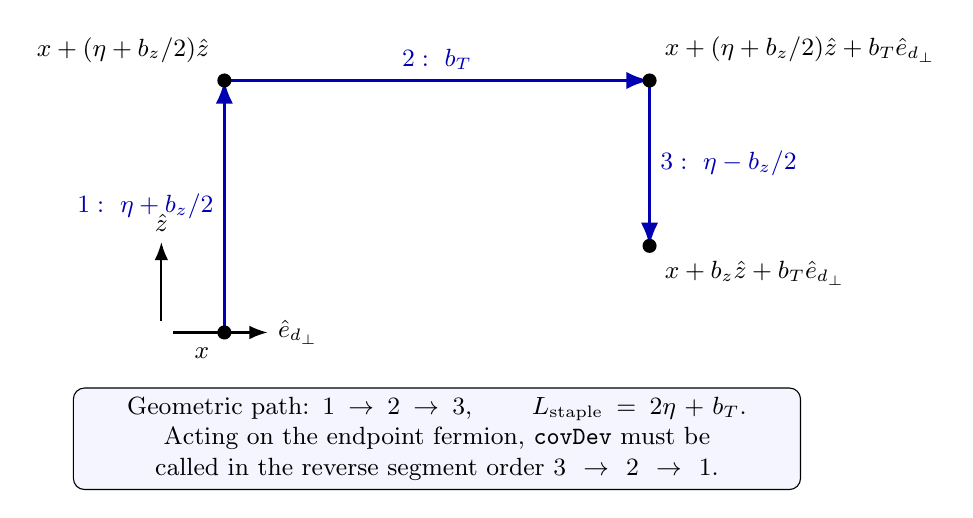
\begin{tikzpicture}[
      >=Latex,
      path/.style={->, very thick, blue!70!black},
      point/.style={circle, fill=black, inner sep=1.8pt},
      label/.style={font=\small, align=center}
    ]
    \coordinate (p0) at (0,0);
    \coordinate (p1) at (0,3.2);
    \coordinate (p2) at (5.4,3.2);
    \coordinate (p3) at (5.4,1.1);

    \draw[path] (p0) -- node[left, label]
      {$1:\ \eta+b_z/2$} (p1);
    \draw[path] (p1) -- node[above, label]
      {$2:\ b_T$} (p2);
    \draw[path] (p2) -- node[right, label]
      {$3:\ \eta-b_z/2$} (p3);

    \node[point] at (p0) {};
    \node[point] at (p1) {};
    \node[point] at (p2) {};
    \node[point] at (p3) {};

    \node[label, below left=2pt and 2pt of p0] {$x$};
    \node[label, above left=3pt and 2pt of p1]
      {$x+(\eta+b_z/2)\hat z$};
    \node[label, above right=3pt and 2pt of p2]
      {$x+(\eta+b_z/2)\hat z+b_T\hat e_{d_\perp}$};
    \node[label, below right=2pt and 2pt of p3]
      {$x+b_z\hat z+b_T\hat e_{d_\perp}$};

    \draw[->, thick] (-0.8,0.15) -- (-0.8,1.15)
      node[above, label] {$\hat z$};
    \draw[->, thick] (-0.65,0) -- (0.55,0)
      node[right, label] {$\hat e_{d_\perp}$};

    \node[
      draw,
      rounded corners,
      fill=blue!4,
      label,
      text width=9.0cm
    ] at (2.7,-1.35) {
      Geometric path: $1\rightarrow2\rightarrow3$,
      \qquad $L_{\rm staple}=2\eta+b_T$.\\
      Acting on the endpoint fermion, \texttt{covDev} must be called in
      the reverse segment order $3\rightarrow2\rightarrow1$.
    };
  \end{tikzpicture}
  \caption{Fixed-length GI qTMD staple geometry, drawn for a representative
  positive $b_z$.  Segment 3 has signed displacement
  $(b_z/2-\eta)\hat z$; its displayed downward length is
  $\eta-b_z/2$.  The same formulas cover negative $b_z$.}
  \label{fig:gi_qtmd_staple}
\end{figure}

Figure~\ref{fig:gi_qtmd_staple} distinguishes the geometric path from the
operator-composition order.  With
$D_\mu\psi(x)=U_\mu(x)\psi(x+\hat\mu)$, the rightmost displacement acts on
the endpoint field first, so the implementation traverses the segment list in
reverse when constructing the transporter.

Thus the total staple length is
\begin{equation}
  L_{\rm staple} = 2\eta + b_T,
\end{equation}
independent of $b_z$.  This is useful for renormalization studies because
different even $b_z$ values at fixed $\eta$ and $b_T$ share the same total
staple length.  The constraints are
\begin{equation}
  b_z \in 2\mathbb{Z}, \qquad \eta \geq \frac{|b_z|}{2}, \qquad b_T \geq 0.
\end{equation}

The implementation uses the same tested neutral helper convention as the
disconnected qTMD one-point code: first build reusable gauge-only staple
transporters, then apply each transporter to the endpoint-shifted forward
propagator.  The shared \texttt{qtmd\_operator\_utils.py} interface contains
\begin{itemize}[nosep]
  \item \texttt{create\_gi\_qtmd\_wilsonline\_index\_lists(...)},
  \item \texttt{build\_gi\_qtmd\_staple\_links(...)},
  \item \texttt{apply\_gi\_qtmd\_staple\_to\_propagator(...)}.
\end{itemize}

The HDF5 tag for the connected pion gauge-invariant staple output is
\texttt{GI\_qTMD.ex}.  The HDF5 internal path still uses the existing qTMD
writer convention
\begin{equation}
  b_X/\eta\eta/bT b_T
  \quad \text{or} \quad
  b_Y/\eta\eta/bT b_T,
\end{equation}
with the full $W$ list saved by the writer.  For the local/PDF sanity limits,
the expected equality is
\begin{equation}
  C_3^{\rm GI\_qTMD}(b_T=0,\; b_z=\pm 2\eta,\; \eta)
  =
  C_3^{\rm GI\_PDF}(b_z=\pm 2\eta),
\end{equation}
up to the common momentum, gamma, source, and sink conventions.

The corrected composition order was validated on the repository
\texttt{S8T8\_wilson\_b6.0} gauge after one production-style four-dimensional
HYP step.  One-rank (\texttt{1.1.1.1}) and four-rank (\texttt{2.2.1.1}) runs
gave bitwise-identical gathered staple fields.  Across positive and negative
$b_z$, both transverse directions, and the straight-PDF limits, the largest
cached-versus-direct relative $L_2$ error was $3.62\times10^{-16}$.  Field
covariance, cached-link endpoint covariance, and contracted-loop gauge
invariance were all below $4.08\times10^{-16}$ in relative $L_2$ error, while
the link-free coordinate-shift control changed by $0.29$--$0.96$.  The former
segment order differs from the corrected result by $0.438$--$0.675$ on the
non-straight actual-gauge paths.  A minimal connected GI-qTMD comparison
produced the same 16 HDF5 files and 192 datasets in both layouts; its maximum
dataset relative $L_2$ difference was $1.31\times10^{-13}$, maximum absolute
difference was $1.42\times10^{-16}$, and maximum solver true residual was
$8.54\times10^{-16}$.

\begin{center}
\begin{tabular}{c|c|l}
\hline
\textbf{Field} & \textbf{Values} & \textbf{Meaning} \\ \hline
$b_T$      & $0,1,\dots,b_T^{\rm max}$ & Transverse displacement \\
$b_z$      & $-b_z^{\rm max},\dots,+b_z^{\rm max}$ & Longitudinal displacement; even for GI qTMD \\
$\eta$      & $0$ for CG, $\eta \ge |b_z|/2$ for GI qTMD & Staple length parameter \\
direction  & $0$ or $1$ & $0$ for $x$, $1$ for $y$ \\
\hline
\end{tabular}
\end{center}

\begin{thebibliography}{9}

\bibitem{Ji:2013dva}
X.~Ji,
\emph{Parton Physics on a Euclidean Lattice},
Phys.\ Rev.\ Lett.\ \textbf{110}, 262002 (2013),
arXiv:1305.1539 [hep-ph].

\bibitem{Ji:2014gla}
X.~Ji,
\emph{Parton Physics from Large-Momentum Effective Field Theory},
Sci.\ China Phys.\ Mech.\ Astron.\ \textbf{57}, 1407--1412 (2014),
arXiv:1404.6680 [hep-ph].

\bibitem{Ji:2020ect}
X.~Ji, Y.-S.~Liu, Y.~Liu, J.-H.~Zhang, and Y.~Zhao,
\emph{Large-Momentum Effective Theory},
Rev.\ Mod.\ Phys.\ \textbf{93}, no.~3, 035005 (2021),
arXiv:2004.03543 [hep-ph].

\bibitem{Radyushkin:2017cyf}
A.~V.~Radyushkin,
\emph{Quasi-parton distribution functions, momentum distributions, and
pseudo-parton distribution functions},
Phys.\ Rev.\ D \textbf{96}, 034025 (2017),
arXiv:1705.01488 [hep-ph].

\bibitem{Orginos:2017kos}
K.~Orginos, A.~Radyushkin, J.~Karpie, and S.~Zafeiropoulos,
\emph{Lattice QCD exploration of parton pseudo-distribution functions},
Phys.\ Rev.\ D \textbf{96}, 094503 (2017),
arXiv:1706.05373 [hep-ph].

\end{thebibliography}

\end{document}
